\documentclass[12pt]{article}

\usepackage[utf8]{inputenc}
\usepackage[T1]{fontenc}
\usepackage[catalan]{babel}
\usepackage{lmodern}
\usepackage{geometry}
\usepackage{hyperref}
\usepackage[dvipsnames]{xcolor}
\usepackage[bf,sf,small,pagestyles]{titlesec}
\usepackage{titling}
\usepackage[font={footnotesize, sf}, labelfont=bf]{caption} 
\usepackage{siunitx}
\usepackage{graphicx}
\usepackage{booktabs}
\usepackage{amsmath,amssymb}
\usepackage[catalan,sort]{cleveref}
\usepackage{enumitem}

\geometry{
	a4paper,
	right = 2.5cm,
	left = 2.5cm,
	bottom = 3cm,
	top = 3cm
}

\hypersetup{
	colorlinks,
	linkcolor = {red!50!blue},
	linktoc = page
}

\crefname{figure}{figura}{figures}
\crefname{table}{taula}{taules}

\graphicspath{{./figs/}}

% Unitats
\sisetup{
	inter-unit-product = \ensuremath{ \cdot },
	allow-number-unit-breaks = true,
	detect-family = true,
	list-final-separator = { i },
	list-units = single
}

\newcommand{\Z}{\mathbb{Z}}
\renewcommand{\vec}[1]{\mathbf{#1}}
\newcommand{\N}{\mathbb{N}}
\newcommand{\R}{\mathbb{R}}
\newcommand{\C}{\mathbb{C}}
\newcommand{\Ry}{\mathit{Ry}}
\let\Im\relax
\let\Re\relax
\DeclareMathOperator{\Im}{Im}
\DeclareMathOperator{\Re}{Re}
\newcommand{\abs}[1]{\lvert #1 \rvert}
\newcommand{\inn}[2]{\left\langle #1 , #2 \right\rangle}
\newcommand{\parbreak}{
	\begin{center}
		--- $\ast$ ---
	\end{center} 
}
\makeatletter
\newcommand*{\defeq}{\mathrel{\rlap{%
    \raisebox{0.3ex}{$\m@th\cdot$}}%
  \raisebox{-0.3ex}{$\m@th\cdot$}}%
	=
}
\makeatother

\newpagestyle{pagina}{
	\headrule
	\sethead*{\sffamily {\bfseries Seminari 1}}{}{\theauthor}
	\footrule
	\setfoot*{}{}{\sffamily \thepage}
}
\renewpagestyle{plain}{
	\footrule
	\setfoot*{}{}{\sffamily \thepage}
}
\pagestyle{pagina}

\title{\sffamily {\bfseries Seminari 1}}
\author{\sffamily Arnau Mas}
\date{\sffamily 25 de març de 2019}

\begin{document}
\maketitle

\section*{Problema 1}
Donada una funció \( H \in C^2(\R^2, \R) \) podem definir dos sistemes d'equacions diferencials al pla. D'una banda el \emph{sistema Hamiltonià},
\begin{equation*}
	\left\{ 
		\begin{aligned}
			\dot{x} & = -\partial_y H(x,y) \\
			\dot{y} & = \partial_x H(x,y),
		\end{aligned} 
	\right. 
\end{equation*}
i de l'altra el \emph{sistema gradient}, 
\begin{equation*}
	\left\{ 
		\begin{aligned}
			\dot{x} & = \partial_x H(x,y) \\
			\dot{y} & = \partial_y H(x,y).
		\end{aligned} 
	\right. 
\end{equation*}

\begin{enumerate}[label=(\roman*), font=\bfseries \sffamily, wide, labelwidth=!, labelindent=0pt]
	\item	És clar que si \( p \in \R^2 \) és un punt crític per un sistema Hamiltonià també ho és pel corresponent sistema gradient, i viceversa, ja que en ambdós casos es té \( \partial_x H(p) = \partial_y H(p) = 0 \). Anem a veure, doncs, que si \( p \) és punt crític per a qualsevol dels dos sistemes ho és per l'altre.   

		El determinant d'una matriu quadrada qualsevol és el producte de les arrels del seu polinomi característic ---si són complexes aleshores són conjugades i per tant el seu producte és real---. Si la matriu diagonalitza ---tant a \( \R \) com a \( \C	\)--- això és el producte dels seus dos valors propis. I si no diagonalitza és el quadrat del seu únic valor propi. 

		El determinant de la diferencial d'ambdós sistemes al punt \( p \) és
		\begin{equation*}
			- \partial_{xy}H(p)^2 + \partial_{xx}H(p) \partial_{yy}H(p).
		\end{equation*}
		Així doncs, si denotem els valors propis de la diferencial del sistema Hamiltonià (potencialment repetits) per \( \lambda_1, \lambda_2 \in \C \), i els corresponents valors propis del sistema gradient per \( \mu_1, \mu_2 \in \C \) tenim
		\begin{equation*}
			\lambda_1 \lambda_2 = \mu_1 \mu_2.
		\end{equation*}
		Per tant \( p \) és punt crític del sistema Hamiltonià si i només si \( \lambda_1 \lambda_2 \neq 0 \), és a dir, si i només si \( \mu_1 \mu_2 \neq 0 \), per tant si i només si és punt crític del sistema gradient. 

	\item Per \( H(x,y) = 2y^2 - y^4 - 2x^2 + 3 \) aleshores el sistema Hamiltonià és 
		\begin{equation}\label{eq:hamiltonia}
			\left\{ 
				\begin{aligned}
					\dot{x} & = 4y^3 - 4y \\
					\dot{y} & = -4x,
				\end{aligned} 
			\right. 
		\end{equation}
		i el sistema gradient és 
		\begin{equation}\label{eq:gradient}
			\left\{ 
				\begin{aligned}
					\dot{x} & = -4x \\
					\dot{y} & = 4y - 4y^3.
				\end{aligned} 
			\right. 
		\end{equation}

		Per determinar el retrat de fase del sistema Hamiltonià hem d'estudiar com són les corbes de nivell de \( H \). Si \( H(x, y) = k \) aleshores
		\begin{equation*}
			x^2 = y^2\left(1 - \tfrac{1}{2}y^2\right) + K,
		\end{equation*}
		amb \( K = \frac{3-k}{2} \). A la \cref{fig:valors del hamiltonia} hi ha representades les funcions \( F_K(y) = y^2\left(1 - \tfrac{1}{2}y^2\right) + K \) per diferents valors de \( K \).
		
		\begin{figure}[htb]
			\centering \sffamily \small
			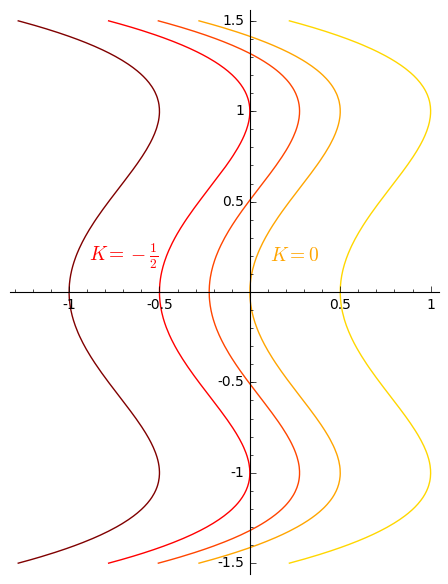
\includegraphics[scale = 0.7]{hamiltonia}
			\caption{La funció \( F_K(y) \) per a diferents valors de \( K \)}
			\label{fig:valors del hamiltonia}
		\end{figure}
		
		Els conjunts de nivell són els que satisfan \( x^2 = F_K(y) \).  Tal i com podem veure a la \cref{fig:valors del hamiltonia}, per a \( K < - \tfrac{1}{2} \) els conjunts de nivells són buits ja que \( F_K(y) < 0j \). Per a \( K = - \frac{1}{2} \)	el conjunt de nivell són exactament dos punts, que són \( (0,1) \) i \( (0,-1) \) i que per tant són dos punts crítics. Per a \( - \frac{1}{2} < K < 0 \) els conjunts de nivell són dues corbes tancades disjuntes, cada una envoltant un dels dos punts crítics que hem trobat. Això dóna lloc a dues òrbites periòdiques disjuntesj. Per a \( K = 0 \) apareix un nou punt crític a l'origen quan les dues corbes disjuntes passen a tocar-se i les dues òrbites periòdiques que teniem abans donen lloc a un parell d'òrbites homoclíniques que neixen i moren a l'origen. Finalment, per a \( K > 0 \) els conjunts de nivell passen a ser corbes tancades que donen lloc a òrbites periòdiques.  

		\begin{figure}[htb]
			\centering \sffamily \small
			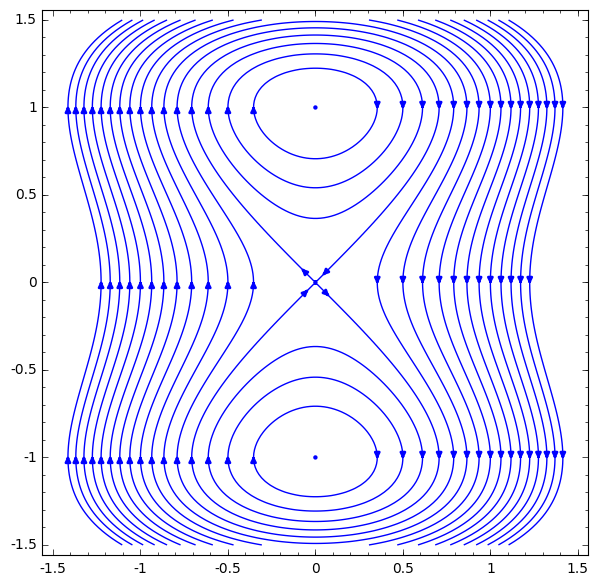
\includegraphics[scale = 0.7]{retrat-hamiltonia}
			\caption{Retrat de fase del sistema Hamiltonià}
			\label{fig:retrat de fase hamiltonia}
		\end{figure}

		Els únics punts crítics del sistema són \( (0,1) \), \( (0,0) \) i \( (0, -1) \). Si calculem els valors del camp en alguns punts ja podem conèixer el retrat de fase ja que com que totes les òrbites tret el parell d'òrbites homoclíniques són periòdiques només ens queda conèixer-ne el sentit de gir. Així obtenim el retrat de fase que es mostra a la \cref{fig:retrat de fase hamiltonia}. Observem que \( (0,1) \) i \( (0, -1) \) són centres mentre que \( (0,0) \) és una sella. 

		Per a determinar el retrat de fase del sistema gradient, observem primer que els eixos i les rectes \( y = 1 \), \( y = -1 \) són invariants. A més \( (0,1) \), \( (0,0) \) i \( (0, -1) \) són els únics punts crítics del sistema. Com que \( \dot{x} > 0 \) sempre que \( x < 0 \) i \( \dot{x} < 0 \) quan \( x > 0 \), la dinàmica sobre l'eix horitzontal és la d'un sistema amb un atractor a l'origen. Sobre l'eix vertical, però, per \( \abs{y} < 1 \), \( \dot{y} \) i \( y \) tenen el mateix signe ---puix que \( \abs{y}^3 < \abs{y} \) quan \( \abs{y} < 1 \), de manera que l'origen és una sella. Pel que fa als altres dos punts crítics, només hem de saber com és la dinàmica a l'eix vertical per \( \abs{y} > 1 \), i en aquestes condicions \( y \) i \( \dot{y} \) tenen signes oposats, de manera que ambdós punts són nodes atractors. 

		La resta d'òrbites queden determinades per continuïtat, i per tant el retrat de fase és el de la \cref{fig:retrat de fase gradient}.

		Veiem que els dos sistemes tenen els mateixos punts crítics. Els nodes atractors del sistema gradient es corresponen amb els centres del sistema hamiltonià, i la sella del sistema gradient es converteix en una sella al sistema hamiltonià. A més, les trajectòries d'un sistema sempre tallen les de l'altre perpendicularment. Això és perquè els seus vectors tangents són perpendiculars. En efecte, si \( \phi \) és una solució del sistema gradient i \( \psi \) és una solució del sistema hamiltonià que es tallen en algun moment, és a dir, hi ha \( t, s \in \R \) tals que \( \phi(t) = \psi(s) \) aleshores
		\begin{equation*}
			\inn{\dot{\phi(t)}}{\dot{\psi(s)}} = \inn{(\partial_x H(\phi(t)), \partial_y H(\phi(t))}{(- \partial_y H(\psi(s)), \partial_x H(\psi(s))} = 0.
		\end{equation*}
		

		\begin{figure}[htb]
			\centering \sffamily \small
			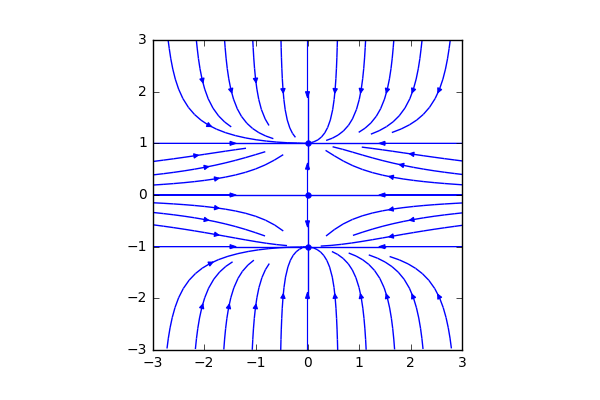
\includegraphics{retrat-gradient}
			\caption{Retrat de fase del sistema gradient}
			\label{fig:retrat de fase gradient}
		\end{figure}

	\item Podem donar una expressió de la varietat estable del sistema Hamiltoniá fent servir que és la corva de nivell \( H(0,0) = 3 \), és a dir, la corba donada per l'equació implícita
		\begin{equation} \label{eq:exacta}
			2y^2 - 2x^2 - y^4 = 0.
		\end{equation}

		D'altra banda, si en un entorn de 0 tenim que la varietat estable és el gràfic d'una funció \( f \colon \R \to \R \) aleshores ha de passar que el flux sobre els punts \( (x, f(x)) \) ha de ser invariant. Una manera d'expressar això és mitjançant la condició
		\begin{equation} \label{eq:condicio}
			\inn{(-f'(x), 1)}{(4f(x)^3 - 4f(x), -4x)} = 0.
		\end{equation}
		En general, si tenim un camp vectorial al pla \( X \colon \R^2 \to \R^2 \) i busquem l'equació d'una corba invariant pel flux del pla, \( y = f(x) \) ha de passar que a tot punt \( p \), \( X(p) \) sigui tangent a la corba. Equivalentment, si considerem la funció \( G(x,y) = y - f(x) \), el seu gradient \( \nabla G \) i \( X \) han de ser ortogonals a tot punt \( (x, f(x)) \). És a dir
		\begin{equation*}
			0 = \inn{\nabla G(x, f(x))}{X(x, f(x))} = \inn{(-f'(x), 1)}{X(x, f(x))},
		\end{equation*}
		que esdevé l'\cref{eq:condicio} en el cas del sistema Hamiltonià que estem considerant.

		Si desenvolupem \( f \) en sèrie de Taylor al voltant de \( 0 \) fins a ordre 2 tenim
		\begin{equation*}
			f(x) = f(0) + f'(0)x + \frac{1}{2}f''(0)x^2 + O(x^3) = ax + \frac{1}{2}bx^2 + O(x^2),
		\end{equation*}
		on hem fet servir que \( f(0) = 0 \), ja que la varietat estable ha de passar per \( (0,0) \), i hem introduït \( a \) i \( b \) per comoditat. Aleshores, substituint a l'\cref{eq:condicio} i ignorant termes d'ordre cúbic o superior obtenim
		\begin{align*}
			0 & = \inn{(-(a + bx) + O(x^3), 1)}{\left(4\left(ax + \tfrac{1}{2}bx^2 + O(x^3)\right)^3 - 4\left(ax + \tfrac{1}{2}bx^2 + O(x^3)\right), -4x\right)} \\
				& = (a + bx)(4ax + 2bx^2 + O(x^3)) - 4x = (4a^2 - 4)x + 6abx^2 + O(x^3).
		\end{align*}
		Per tant hem de tenir \( a^2 = 1 \) i \( b = 0 \). Això dóna lloc a dos valors per \( a \), 1 i \( -1 \). Com podem veure a la \cref{fig:retrat de fase hamiltonia}, la varietat estable i insetable de fet són la mateixa, i els dos possibles valors d'\( a \) es corresponen a les dues branques de la varietat a l'origen. Pel cas de la varietat estable veiem que \( a  = 1 \). Per tant la varietat estable, fins a ordre quadràtic, és
		\begin{equation*}
			y = x + O(x^3). 
		\end{equation*}

		Podem trobar aquests coeficients directament a partir de l'expressió exacta de la varietat estable a l'\cref{eq:exacta}. Si aïllem \( x \) en termes de \( y \) aleshores tenim
		\begin{equation*}
			x = \pm \sqrt{y^2 - \tfrac{1}{2} y^4}. 
		\end{equation*}
		El que hem obtingut, doncs, és una expressió per a \( f^{-1} = g \) que és vàlida en un entorn de \( (0,0) \) ---ja veiem que per exemple cal que \( \abs{y} < \sqrt{2} \)---. L'ambigüitat té a veure amb el fet que pel \( (0,0) \) hi passen tant la varietat estable com inestable, i que ambdues satisfan l'\cref{eq:exacta}. Tal i com veiem al retrat de fase, \cref{fig:retrat de fase hamiltonia}, hem de triar el signe positiu. Si derivem una vegada obtenim
		\begin{equation*}
			g'(y) = \frac{2y - 2y^3}{2\sqrt{y^2 - \tfrac{1}{2}y^4}} = \frac{1 - y^2}{\sqrt{1 - \frac{1}{2}y^2}}
		\end{equation*}
		de manera que \( g(0) = 1 \). I per tant 
		\begin{equation*}
			f'(0) = \frac{1}{(f^{-1})'(f(0))} = \frac{1}{g'(0)} = 1.
		\end{equation*}

		Per trobar el següent terme derivem \( g \) dues vegades per obtenir
		\begin{equation*}
			g''(y) = - \frac{2y}{\sqrt{1 - \tfrac{1}{2}y^2}} + \frac{y}{2\left(1 - \tfrac{1}{2}y^2\right)^{\frac{3}{2}}}.
		\end{equation*}
		Per tant \( g''(0) = 0 \). I aleshores
		\begin{equation*}
			f''(0) = - \frac{(f^{-1})''(0)}{((f^{-1})'(0))^3} = 0,
		\end{equation*}
		que és el resultat que hem obtingut prèviament. 

	\item Els sistemes Hamiltonians poden tenir òrbites periòdiques. L'exemple més senzill és el sistema
		\begin{equation*}
			\left\{ 
				\begin{aligned}
					\dot{x} & = -y \\
					\dot{y} & = x,
				\end{aligned} 
			\right. 
		\end{equation*}
		derivat del Hamiltonià \( H(x, y) = \tfrac{1}{2}x^2 + \tfrac{1}{2}y^2 \). Totes les òrbites d'aquest sistema són periòdiques. 

		Els sistemes Hamiltonians, però, no poden tenir cicles límit. Si \( \gamma \) és un cicle límit, aleshores el Hamiltonià del sistema, \( H \), pren el mateix valor \( H_0 \) a tots els punts de \( \gamma \). Aleshores, per definició de cicle límit, hi ha un entorn \( U \) de \( \gamma \) tal que per tot \( x \in U \), l'\( \omega \)-límit (o \( \alpha \)-límit) de l'òrbita \( \phi \) de \( x \) és \( \gamma \). Prenem una successió \( (t_n) \) tal que \( t_n \xrightarrow{n \to \infty} \infty \) i \( \phi(t_n, x) \xrightarrow{n \to \infty} \gamma \), que existeix per definició d'\( \omega \)-límit. Aleshores, fent ús de la continuïtat d'\( H \)
		\begin{equation*}
			\lim_{n \to \infty}{H(\phi(t_n, x))} = H\left(\lim_{n \to \infty}{\phi(t_n, x)}\right) = H_0.
		\end{equation*}
		Per tant, com que el Hamiltonià és constant a tota l'òrbita de \( x \), ha de valer \( H_0 \) ---pel cas de l'\( \alpha \)-límit prenem una successió tal que \( t_n \to -\infty \) i arribem a la mateixa conclusió)---. Així, tenim que el Hamiltonià pren el valor \( H_0 \) a tot \( U \), en contradicció amb el fet que \( H \) és integral primera i per tant no constant en oberts. 

		Els sistemes gradients no poden tenir òrbites periòdiques. Si hi hagués alguna òrbita periòdica aleshores la circulació del camp al llarg d'aquesta seria no nu\l.la. Però això no és possible ja que els camps gradients tenen circulació nu\l.la al llarg de tot camí tancat. Més en detall, si \( \phi(t) \) és una òrbita periòdica de període \( T \) i \( \gamma = \phi((0, T)) \), aleshores \( \phi \) és una parametrització de \( \gamma \). Com que \( \phi \) és una solució del sistema gradient satisfà \( \dot{\phi}(t) = \nabla H(\phi(t)) \) i la circulació del gradient \( \nabla H \) al llarg de \( \gamma \) és
		\begin{equation*}
			\int_{\gamma} \inn{\nabla H}{T} \, ds = \int_{0}^{T} \inn{\nabla H(\phi(t))}{\dot{\phi}(t)} \, dt = \int_0^T \inn{\dot{\phi}(t)}{\dot{\phi}(t)} \, dt > 0.
		\end{equation*}
		Però això no pot ser ja que els camps gradient tenen circulació nu\l.la al llarg de qualsevol corba tancada.

		En particular, com que els camps gradient no poden tenir òrbites periòdiques tampoc no poden tenir cicles límit.
\end{enumerate}

\section*{Problema 2}
Considerem l'equació diferencial 
\begin{equation*}
	\left\{ 
		\begin{aligned}
			\dot{x} & = P_n(x,y) \\
			\dot{y} & = Q_n(x,y),
		\end{aligned} 
	\right. 
\end{equation*}
on \( P_n(x,y) \) i \( Q_n(x,y) \) són polinomis homogenis de grau \( n \). 

\begin{enumerate}[label=(\roman*), font=\bfseries \sffamily, wide, labelwidth=!, labelindent=0pt]
	\item Suposem que hi ha algun punt crític \( (x_0, y_0) \). Aleshores, per tot \( \lambda \in \R \) tenim
		\begin{gather*}
			P_n(\lambda x_0, \lambda y_0) = \lambda^n P(x_0, y_0) = 0, \\
			Q_n(\lambda x_0, \lambda y_0) = \lambda^n Q(x_0, y_0) = 0. 
		\end{gather*}
		Si \( (x_0, y_0) \neq (0,0) \) el que ens diu això és que tots els punts de la recta que passa per l'origen i per \( (x_0, y_0) \) també són crítics. En particular \( (x_0, y_0) \) no pot ser un punt crític aïllat ja que qualsevol entorn seu conté punts d'aquesta recta i per tant conté altres punts crítics. Així, si hi ha algun punt crític aïllat l'única alternativa és que sigui l'origen. 	

	\item Si reescrivim el sistema en coordenades polars obtenim
		\begin{align*}
			\dot{r} & = \frac{x\dot{x} + y \dot{y}}{r} = \frac{xP_n(x,y) + yQ_n(x,y)}{r} \\
							& = \cos{\theta} P_n(r\cos{\theta}, r \sin{\theta}) + \sin{\theta} Q_n(r \cos{\theta}, r \sin{\theta}) \\
							& = r^n  \big[\cos{(\theta)} P_n(\cos{(\theta)}, \sin{(\theta)}) + \sin{(\theta)} Q_n(\cos{(\theta)}, \sin{(\theta)})\big], \\
			\dot{\theta} & = \frac{x\dot{y} - y \dot{x}}{r^2} = \frac{x Q_n(x,y) - y P_n(x,y)}{r^2} \\
									 & = \frac{1}{r} \big[ \cos{(\theta)} Q_n(r \cos{(\theta)}, r \sin{(\theta)}) - \sin{(\theta)} P_n(r \cos{(\theta)}, r \sin{(\theta)})  \big] \\
									 & = r^{n - 1} \big[ \cos{(\theta)} Q_n(\cos{(\theta)}, \sin{(\theta)}) - \sin{(\theta)} P_n(\cos{(\theta)}, \sin{(\theta)})  \big]. 
		\end{align*}

		Buscar rectes invariants del sistema és el mateix que trobar \( \theta^\ast \) que anu\l.lin \( \dot{\theta} \). Observem, a més, que si \( \theta^\ast \) anu\l.la \( \dot{\theta} \) aleshores \( \theta^\ast + \pi \) també, ja \( \sin{(\theta^\ast + \pi)} = - \sin{(\theta^\ast)} \) i el mateix pel cosinus.   

		Sobre una recta invariant, fora de l'origen, tenim que \( r \neq 0 \), i per tant només hem de buscar les solucions de 
		\begin{equation*}
			Q_n(\cos{\theta}, \sin{\theta}) \cos{\theta} - P_n(\cos{\theta}, \sin{\theta}) \sin{\theta} = 0.
		\end{equation*}
		Si definim \( F(\theta) =	Q_n(\cos{\theta}, \sin{\theta}) \cos{\theta} - P(\cos{\theta}, \sin{\theta}) \sin{\theta} \) aleshores tenim que 
		\begin{equation*}
			F(0) = Q_n(1, 0).
		\end{equation*}
		i 
		\begin{equation*}
			F(\pi) = - Q_{n}(-1, 0) = (-1)^{n+1}Q_n(1,0).
		\end{equation*}

		En general, un polinomi homogeni en dues variables es pot escriure
		\begin{equation*}
			P(x,y) = \sum_{k = 0}^n \alpha_k x^k y^{n - k}.
		\end{equation*}
		En particular, \( P(1, 0) = \alpha_n \), i similarment \( P(0,1) = \alpha_0 \). Posem, doncs
		\begin{equation*}
			Q_n(x,y) = \sum_{k = 0}^n \alpha_k x^k y^{n - k},
		\end{equation*}
		i per tant \( F(0) = \alpha_n \) i \( F(\pi) = (-1)^{n+1} \alpha_n \). Si \( n \) és parell aleshores \( F(0) = - F(\pi) \). Si \( \alpha_n = 0 \) aleshores \( F(0) = F(\pi) = 0 \) i per tant l'eix horitzontal és una recta invariant. Si no, per Bolzano \( F \) ha de tenir algun zero entre \( 0 \) i \( \pi \), el qual correspon a una recta invariant. 

		Per tant, per \( n \) parell sempre hi ha rectes invariants. Això implica que no hi poden haver solucions que envoltin l'origen, ja que haurien de creuar les rectes invariants, la qual cosa no és possible. Per tant, per \( n \) parell, l'origen no pot ser ni un centre ni un focus.  

	\item Si \( n \) és senar, aleshores sempre podem trobar un sistema de la mena que estem considerant tal que l'origen és un centre. Un exemple senzill és 
		\begin{equation*}
			\left\{ 
				\begin{aligned}
					\dot{x} & = -y^n \\
					\dot{y} & = x^n,
				\end{aligned} 
			\right. 
		\end{equation*}
		Els sistemes d'aquesta mena són Hamiltonians amb Hamiltonià
		\begin{equation*}
			H(x,y) = \frac{x^{n+1} + y^{n+1}}{n + 1}. 
		\end{equation*}
		Les corbes de nivell d'\( H \), com que \( n \) és parell, són corbes tancades que envolten l'origen. I com que no hi ha més punts crítics que l'origen, totes les òrbites són periòdiques. 

		Més detalladament, si escrivim aquest sistema en coordenades polars aleshores obtenim 
		\begin{equation*}
			\left\{ 
				\begin{aligned}
					\dot{r} & = r^n \big[(\sin{\theta})^n \cos{\theta} - (\cos{\theta})^n \sin{\theta}\big] \\
					\dot{\theta} & = r^{n-1}\big[(\sin{\theta})^{n+1}  + (\cos{\theta})^{n+1} \big],
				\end{aligned} 
			\right. 
		\end{equation*}
		Aleshores \( \dot{\theta} > 0 \) ja que \( n+1 \) és parell. Així totes les solucions han d'envoltar l'origen. Podem calcular \( r(\theta) \) per saber a quina distància de l'origen es troba la solució un cop ha fet una volta. Com que
		\begin{equation*}
		\frac{1}{r}\frac{dr}{d\theta} = \frac{(\sin{\theta})^n \cos{\theta} - (\cos{\theta})^n \sin{\theta}}{(\sin{\theta})^{n+1}  + (\cos{\theta})^{n+1} },
		\end{equation*}
	Si la la coordenada polar inicial és \( \theta_0 \) aleshores
	\begin{equation*}
		\log{\frac{r(\theta_0 + 2\pi)}{r(\theta_0)}} = \int_{\theta_0}^{\theta_0 + 2\pi} \, \frac{(\sin{\psi})^n \cos{\psi} - (\cos{\psi})^n \sin{\psi}}{(\sin{\psi})^{n+1}  + (\cos{\psi})^{n+1} } \, d \psi.
	\end{equation*}
	Per resoldre aquesta integral podem fer el canvi \( u(\psi) = (\sin{\psi})^{n+1}  + (\cos{\psi})^{n+1} \)	i aleshores \( u'(\psi) = -(n+1)\left((\sin{\psi})^n \cos{\psi} - (\cos{\psi})^n \sin{\psi}\right) \). De manera que
	\begin{equation*}
	\log{\frac{r(\theta_0 + 2\pi)}{r(\theta_0)}} = - \frac{1}{n+1} \int_{u(\theta_0)}^{u(\theta_0 + 2\pi)} \frac{1}{u} \, du. 
	\end{equation*}
	Però aquesta integral de fet és nu\l.la ja que \( u(\theta_0 + 2\pi) = u(\theta_0) \). Per tant \( r(\theta_0 + 2\pi) = r(\theta_0) \) de manera que l'òrbita és periòdica i per tant l'origen és un centre. 	
	

		També hi ha sistemes on l'origen és un focus. Un exemple és 
		\begin{equation*}
			\left\{ 
				\begin{aligned}
					\dot{x} & = -y^{2k+1} - x^{k+1} y^{k} \\
					\dot{y} & = x^{2k+1} - y^{k+1}x^k.
				\end{aligned} 
			\right. 
		\end{equation*}
		En coordenades polars el sistema és 
		\begin{equation*}
			\left\{ 
				\begin{aligned}
					\dot{r} & = r^n \big[(\sin{\theta})^n \cos{\theta} - (\cos{\theta})^n \sin{\theta} - (\sin{\theta}\cos{\theta})^k\big] \\
					\dot{\theta} & = r^{n-1}\big[(\sin{\theta})^{n+1}  + (\cos{\theta})^{n+1} \big],
				\end{aligned} 
			\right. 
		\end{equation*}
		on \( n = 2k + 1 \). Com abans, \( \dot{\theta} > 0 \) i les òrbites estan obligades a envoltar l'origen. Si fem el mateix càlcul que abans per determinar a quina distància arriba la trajectòria un cop ha fet una volta trobem
		\begin{align*}
			\log{\frac{r(\theta_0 + 2\pi)}{r(\theta_0)}} & = \int_{\theta_0}^{\theta_0 + 2\pi} \, \frac{(\sin{\psi})^n \cos{\psi} - (\cos{\psi})^n \sin{\psi}}{(\sin{\psi})^{n+1}  + (\cos{\psi})^{n+1} } \, d \psi -  \int_{\theta_0}^{\theta_0 + 2\pi} \, \frac{(\sin{\theta}\cos{\theta})^k}{(\sin{\psi})^{n+1}  + (\cos{\psi})^{n+1} } \, d \psi \\
																									 & = -  \int_{\theta_0}^{\theta_0 + 2\pi} \, \frac{(\sin{\theta}\cos{\theta})^k}{(\sin{\psi})^{n+1}  + (\cos{\psi})^{n+1} } \, d \psi
		\end{align*}
		Si \( k \) és parell, l'integrand d'aquesta integral és sempre positiu i per tant té integral positiva, de manera que \( r(\theta_0) > r(\theta_0 + 2\pi) \) i per tant l'origen és un focus. 
	\item Si el sistema té un centre o un focus aquest ha de ser aïllat. Per tant només pot ser l'origen. L'origen és punt crític de qualsevol sistema d'aquesta mena, ja que els polinomis homogenis sempre satisfan \( P(0,0) = 0 \). 
		
		És clar que si el sistema té un centre o un focus aleshores no pot tenir rectes invariants. Per tant és necessari que no hi hagi rectes invariants. De fet és necessari i suficient. Si no hi ha rectes invariants aleshores \( \dot{\theta} \) no s'anu\l.la mai, de manera que és sempre positiva o sempre negativa. En qualsevol cas, les solucions estan obligades a envoltar a l'origen, ja sigui en un en sentit o en l'altre.

		Per distingir si es tracta d'un centre o un focus, hem de repetir el càlcul de l'apartat anterior. És a dir, l'origen serà un centre si i només si \( r(\theta) \) és \( 2\pi \)-periòdic, i un focus en cas contrari. Per tant tenim un centre si i només si
		\begin{equation*}
			\log{\frac{r(\theta_0 + 2\pi)}{r(\theta_0)}} = \int_{\theta_0}^{\theta_0 + 2\pi} \frac{Q_n(\cos{\psi}, \sin{\psi}) \sin{\psi} + P_n(\cos{\psi}, \sin{\psi}) \cos{\psi}}{Q_n(\cos{\psi}, \sin{\psi}) \cos{\psi} - P_n(\cos{\psi}, \sin{\psi}) \sin{\psi}} \, d\psi = 0,
		\end{equation*}
	i un focus en cas contrari. 	

\end{enumerate}

\section*{Problema 3}
Donada una funció \( H \in C^2(\R^2, \R) \) és molt senzill trobar un sistema d'equacions que la tingui com a integral primera, concretament
\begin{equation*}
	\left\{ 
		\begin{aligned}
			\dot{x} & = -\partial_y H(x,y) \\
			\dot{y} & = \partial_x H(x,y).
		\end{aligned} 
	\right. 
\end{equation*}

Si volem generalitzar això a dimensió 3, donades \( H_1, H_2 \in C^2(\R^2, \R) \) aleshores definim el camp
\begin{equation*}
	X(x, y, z) = \begin{vmatrix}
		\vec{e}_1 & \vec{e}_2 & \vec{e}_3 \\
		\partial_x H_1(x,y,z) & \partial_y H_1(x,y,z) & \partial_z H_1(x,y,z) \\
		\partial_x H_2(x,y,z) & \partial_y H_2(x,y,z) & \partial_z H_2(x,y,z) 
	\end{vmatrix},
\end{equation*}
que és no nul ja que per hipòtesi els gradients de \( H_1 \) i \( H_2 \) són linealment independents. Aleshores el sistema \( \dot{\vec{x}} = X(\vec{x}) \) té a \( H_1 \) i \( H_2 \) per integrals primeres. Una manera de comprovar-ho és veient que \( \inn{X}{\nabla H_1} = \inn{X}{\nabla H_2} = 0 \).  
\begin{align*}
	\inn{X}{\nabla H_1} & = \partial_x H_1 \begin{vmatrix}
		\partial_x H_1 & \partial_y H_1 \\
		\partial_x H_2 & \partial_y H_2 
	\end{vmatrix}
- \partial_y H_1 \begin{vmatrix}
		\partial_x H_1 & \partial_z H_1 \\
		\partial_x H_2 & \partial_z H_2 
	\end{vmatrix}
+ \partial_z H_1 \begin{vmatrix}
		\partial_x H_1 & \partial_y H_1 \\
		\partial_x H_2 & \partial_y H_2 
	\end{vmatrix} \\
	& = \begin{vmatrix}
		\partial_x H_1 & \partial_y H_1 & \partial_x H_1 \\
		\partial_x H_1 & \partial_y H_1 & \partial_x H_1 \\
		\partial_x H_2 & \partial_y H_2 & \partial_x H_2 
	\end{vmatrix} = 0.
\end{align*}
El càlcul per \( H_2 \) és essencialment igual.  

La generalització a dimensión \( n \) és clara. Donades \( H_1, \dots, H_{n-1} \in C^2(\R^{n}, \R) \) definim el camp
\begin{equation} \label{eq:determinant}
	X(\vec{x}) = \begin{vmatrix}
		\vec{e}_1 & \cdots & \vec{e}_n \\
		\partial_1 H_1(\vec{x}) & \cdots & \partial_n H_1(\vec{x}) \\
		\vdots & \ddots & \vdots \\ 
		\partial_1 H_{n-1}(\vec{x}) & \dots & \partial_n H_{n-1}(\vec{x}) 
	\end{vmatrix},
\end{equation}
on \( \partial_k H \) és la parcial d'\( H \) respecte la \( i \)-èssima coordenada.

Aleshores, si denotem els menors del determinant de l'\cref{eq:determinant} per \( A_{i,k} \)
\begin{align*}
	\inn{X(\vec{x})}{\nabla H_i(\vec{x})} & = \sum_{k = 1}^n (-1)^k \partial_k H_i(\vec{x}) A_{i,k} \\
																				& = \begin{vmatrix}
		\partial_1 H_i(\vec{x}) & \cdots & \partial_n H_i(\vec{x}) \\
		\partial_1 H_1(\vec{x}) & \cdots & \partial_n H_1(\vec{x}) \\
		\vdots & \ddots & \vdots \\ 
		\partial_1 H_{n-1}(\vec{x}) & \dots & \partial_n H_{n-1}(\vec{x}) 
	\end{vmatrix} = 0,
\end{align*}
De manera que \( H_1, \dots, H_n \) són integrals primeres del sistema.

\end{document}

